\section{Facebook's Foundational Integrity Research Award on Misinformation and Polarization}
\label{sec:deep}
%\pagestyle{plain}
\begin{landscape}
%                     PI      Uni     Pos    Proj   Amoun    Disclosed   
\begin{longtable}[c]{|L{2.5cm}|L{3cm}|L{2cm}|L{5cm}|C{1.7cm}|C{1.3cm}|C{2.5cm}|}
\hline
\multicolumn{7}{|c|}{\sffamily Facebook's Foundational Integrity Research Award on \textit{Misinformation and Polarization}} \tabularnewline
\hline
{\sffamily\small Researcher} & {\sffamily\small University} & {\sffamily\small Position} &{\sffamily\small Project Title} & {\sffamily\small Amount} & {\sffamily\small On CV} & {\sffamily\small Dubious Topic} \tabularnewline
\hline
\hline
\endfirsthead
\hline
{\sffamily\small Researcher} & {\sffamily\small University} & {\sffamily\small Position} &{\sffamily\small Project Title} & {\sffamily\small Amount} & {\sffamily\small On CV} & {\sffamily\small Dubious Topic} \tabularnewline
\hline
\hline
\endhead
Ayesha Ali\footnote{Already received a Facebook Research Award over \$50'000 on: \textit{Understanding the Impact of Digital Literacy on Misinformation in Pakistan}.} & Lahore University of Management Sciences & Assistant Professor-Tenure Track & Countering deepfake misinformation among low digital-literacy populations & \$90'000 & YES &  \tabularnewline\hline
Brandon Stewart & Princeton University & Assistant Professor & Do online video recommendation algorithms increase affective polarization? & N/A & N/A &  \tabularnewline\hline
Bronwyn Carlson & Macquarie University & Head of Department & Indigenous women and LBGTQI+ people and violence on Facebook & N/A & NO &  \tabularnewline\hline
Denis Stukal & University of Sydney & Lecturer & Unpacking trust and bias in social media news in developing countries & \$86'000 & YES &  \tabularnewline\hline
Erik C. Nisbet & Northwestern University & Associate Professor & Quantifying harms of misinformation during the U.S. presidential election & N/A & NO &  \tabularnewline\hline
Godfred Bokpin & CUTS Accra & Professor & Do users in India, Kenya, Ghana react differently to problematic content? & N/A & N/A & No relation to polarisation or misinformation \tabularnewline\hline
Fei Shen & City University of Hong Kong & Associate Professor & Can third party fact-checkers on Facebook reduce affective polarization? & \$85'000 & YES &  \tabularnewline\hline
Heidi Larson & London School of Hygiene \& Tropical Medicine & Professor & The contagion of misinformation & N/A & YES \footnote{* Disclosed on the homepage or a closely related site.}\textsuperscript{*} & Strong focus on private messaging \footnote{While relevant for FB messenger and WhatsApp, this has little to do with what Facebook announced as topic of the award.} \tabularnewline\hline
Joanne Lloyd & University of Wolverhampton & Senior Lecturer & Exploring harmful [mis]information via normalized online violent content & N/A & YES\textsuperscript{*} &  \tabularnewline\hline
Joseph W. Kable & University of Pennsylvania & Professor & Quantifying persistent effects of misinformation via neural signals & N/A & NO\footnote{$\dagger$ Outdated}\textsuperscript{$\dagger$} & Not addressing the topic that Facebook promoted publicly \tabularnewline\hline
Justin Kalisti Urassa & Sokoine University of Agriculture & Associate Professor & Digital literacy and misinformation among smallholder farmers in Tanzania & N/A & NO\textsuperscript{$\dagger$} &  \tabularnewline\hline
Kathryn Cottingham & Dartmouth College & Professor  & Micro-Influencers as digital community health workers & N/A & YES\textsuperscript{*} & Very specific, potential talking point for Facebook \tabularnewline\hline
Kevin Munger & Pennsylvania State University & Assistant Professor & Digital literacy in Latin America: Developing measures for WhatsApp & \$100'000 & YES\footnote{Without topic} & \tabularnewline\hline
Lucas Calil Guimarães Silva & Fundação Getúlio Vargas & Researcher & The circulation of dangerous speech in the 2020 Brazilian elections & N/A & N/A &  \tabularnewline\hline
Marta Barbara Ochman & Instituto Tecnológico y de Estudios Superiores de Monterrey & Core Researcher & Affective polarization and contentious politics: Women’s movement in Mexico & N/A & NO\footnote{The project is listed however without mentioning Facebook.} &  \tabularnewline\hline
Meghan Sobel Cohen & Regis University & Associate Professor         & Digital literacy in East Africa: A three country comparative study & N/A & N/A & No relation to polarisation or misinformation \tabularnewline\hline
Mercy Fekadu Mulugeta & Addis Ababa University & Academic Director  & Dangerous speech, social media and violence in Ethiopia & N/A & N/A & \tabularnewline\hline
Michael Bang Petersen & Aarhus University & Full Professor & Cross-cultural psychological motivations of online political hostility & N/A & NO\textsuperscript{$\dagger$} &  \tabularnewline\hline
Natália Salgado Bueno & Emory University & Assistant Professor & Political elites and the appeal of fake news in Brazil & \$74'970 & YES\footnote{In a paper on \emph{Motivated Reasoning Without Partisanship? Fake News in the 2018 Brazilian Elections} which is as of \today under revision, the authors did not disclose any research finding. The work is clearly attributable to the Facebook Research Award: there is very close relation to the topic and the authors are the exact same group of researchers who received the grant. The paper is as of today available at \url{https://www.abcp2020.sinteseeventos.com.br/arquivo/downloadpublic?q=YToyOntzOjY6InBhcmFtcyI7czozNToiYToxOntzOjEwOiJJRF9BUlFVSVZPIjtzOjQ6IjM1MjQiO30iO3M6MToiaCI7czozMjoiZjRiNDQ3YmVkMTljNTVjOWQ1Y2Q5NDdhNDBkM2NjMDQiO30\%3D}} & \tabularnewline\hline
Nicole Stremlau & University of Oxford & Senior Research Fellow & When online speech meets offline harm: Internet shutdowns in Africa & N/A & N/A & \tabularnewline\hline
Selim Erdem Aytaç & Koç University & Associate Professor & Affective polarization: Causal drivers, online networks, and Interventions & N/A & NO &  \tabularnewline\hline
Sergio Splendore & Universitá degli Studi di Milano & Associate Professor & STOP! Selective trust originates polarization & \$99'750 & YES & N/A \tabularnewline\hline
Shannon C. McGregor & University of North Carolina at Chapel Hill & Assistant Professor & Political identity ownership & N/A & NO\textsuperscript{$\dagger$} & N/A \tabularnewline\hline
Victoria A. Parker & Wilfrid Laurier University & PhD Student & Examining how ingroup dissent on social media mitigates false polarization & \$49'830 \footnote{Disclosed on \url{https://students.wlu.ca/academics/graduate-and-postdoctoral-studies/news/2020/fall/laurier-researchers-selected-as-facebook-award-recipients.html}} & N/A &  \tabularnewline\hline
\end{longtable}
\begin{itemize}
    \item[-] N/A in the column \textit{Amount} indicates that the funding amount was not disclosed.
    \item[-] N/A in the column \emph{On CV} indicates that either no CV was available, no funding information was available, or even that no web presence could be found. 
\end{itemize}
\end{landscape}
%\pagestyle{fancy}

%\section{Further Remarks}
%\label{app:additional_paper}
%For reasons of concision and space I did not include all relevant and influential (i.e. highly cited) studies I found into section \ref{sec:mapping}, but present some sound bites from their papers:

%\citep{mcdaniel_new_2012} A study on well-being of new mothers found: \textquote{In sum, blogging may improve new mothers’ well-being, as they feel more connected to the world outside their home through the Internet.}



%\citep{kross_facebook_2013} \textquote{On the surface, Facebook provides an invaluable resource for fulfilling the basic human need for social connection. Rather than enhancing well-being, however, these findings suggest that Facebook may undermine it.}

%\citep{rosen_is_2013} This study on Facebook use and clinical symptoms of psychiatric disorders finds: \textquote{The results showed both positive and negative aspects of technology including social media as well as apparently detrimental effects of a preference for multitasking.}



%\citep{orben_association_2019} A study on well-being and digital technology use finding: \textquote{Taking the broader context of the data into account suggests that these effects are too small to warrant policy change.}

%\citep{coyne_does_2020}: A Longitudinal study over 8 years with participants filling in a yearly survey: \textquote{Results revealed that increased time spent on social media was not associated with increased mental health issues across development when examined at the individual level.}



\section{Figures}
\label{app:figures}
\begin{figure}
\centering
    \begin{subfigure}[b]{0.83\textwidth}
        \centering
        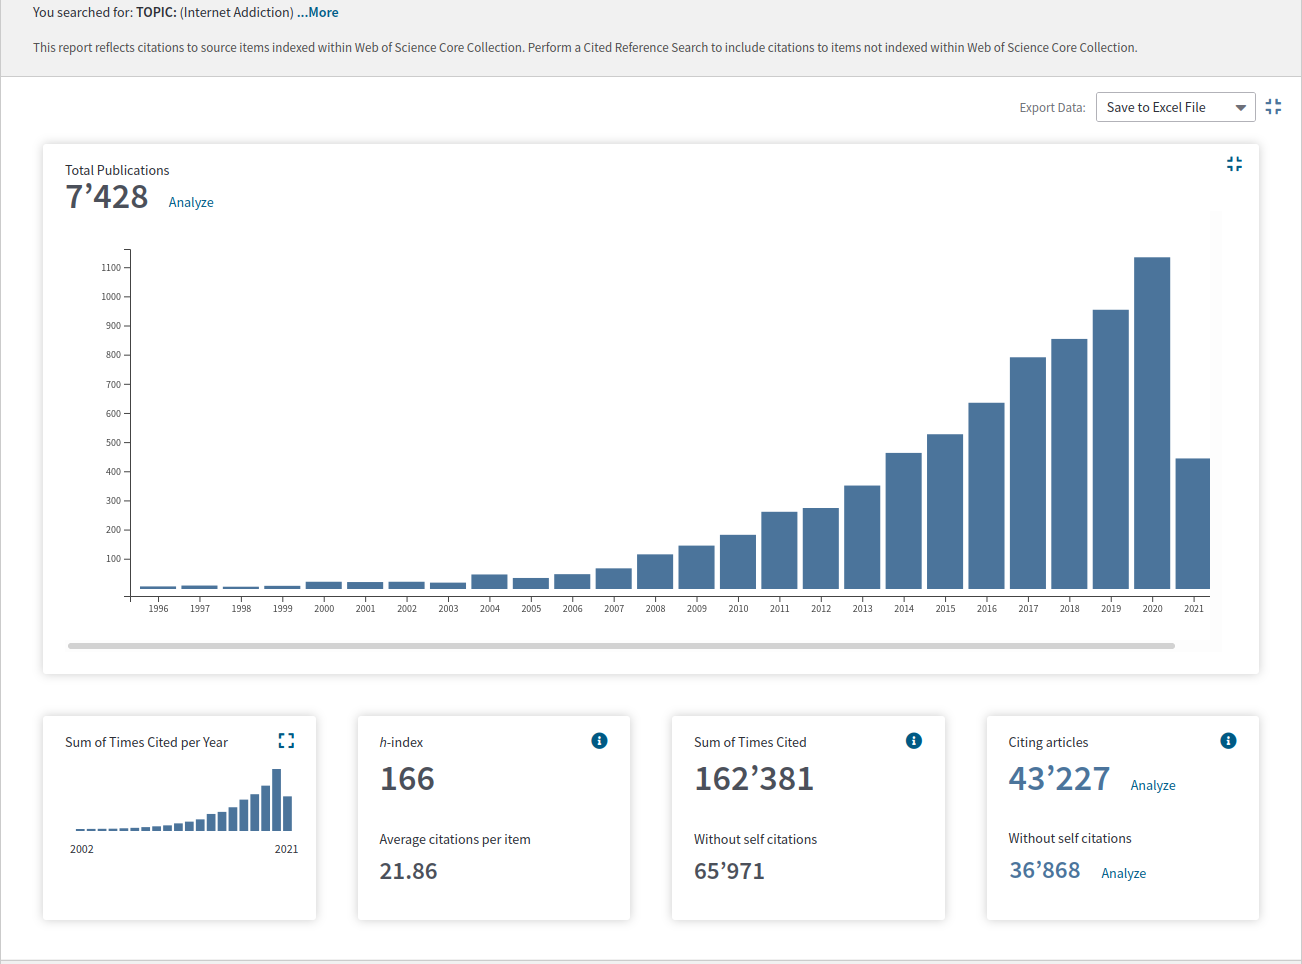
\includegraphics[width = \textwidth]{figures/Internet_addiction.png}
        \caption{The screen-shot of a \href{https://apps.webofknowledge.com/}{Web of Science} citation report created on July 7th, 2021, for the search term \textquote{Internet Addiction}.}
        \label{fig:internet_addiction}
    \end{subfigure}
    \begin{subfigure}[b]{0.83\textwidth}
        \centering
    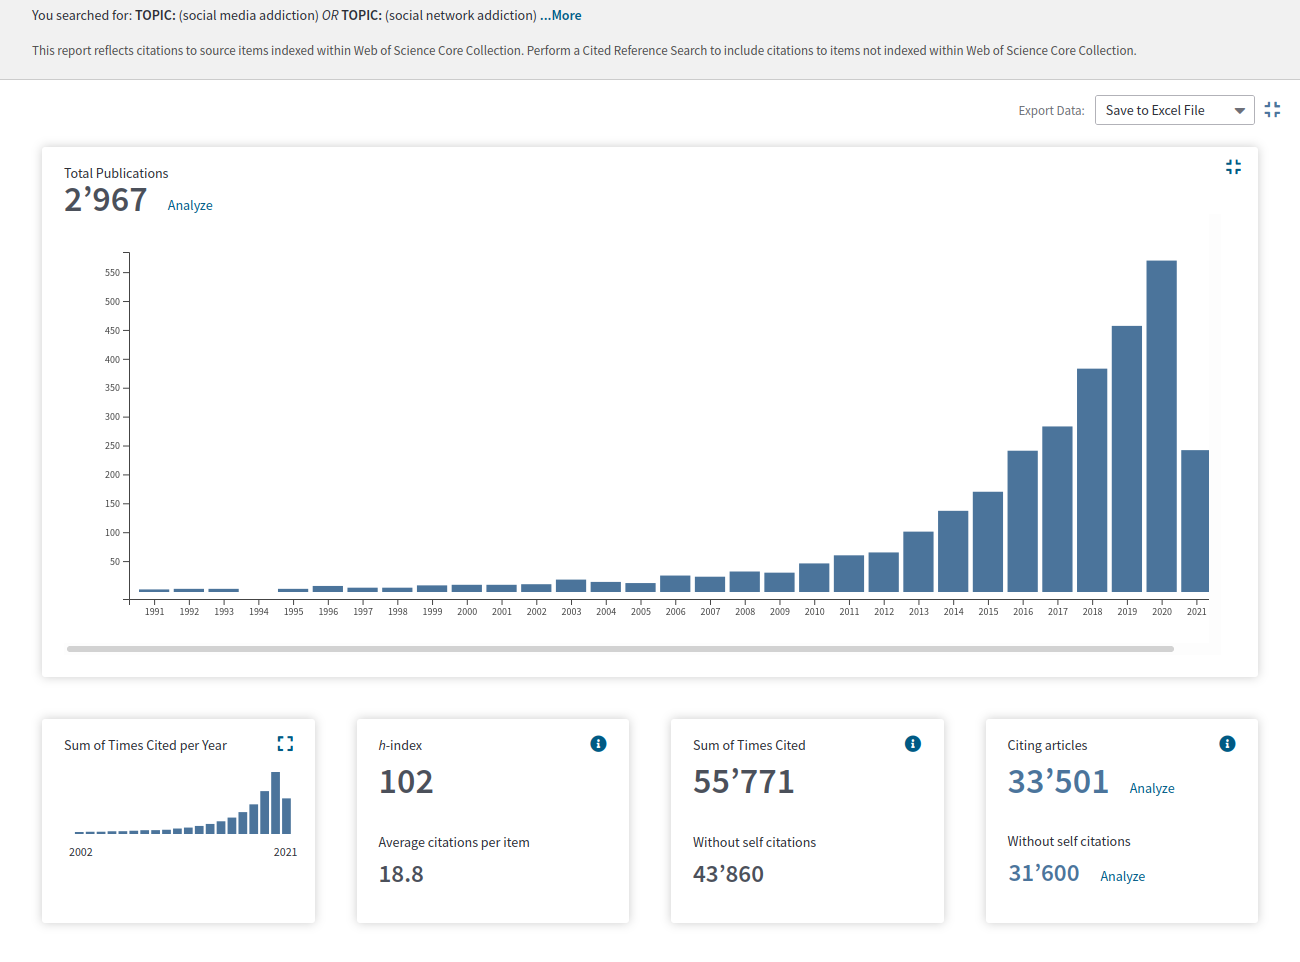
\includegraphics[width = \textwidth]{figures/Social_media_addiction.png}
    \caption{The screen-shot of a \href{https://apps.webofknowledge.com/}{Web of Science} citation report created on July 7th, 2021, for \textquote{TOPIC:(Social Media Addiction) OR TOPCI:(Social Network Addiction)}.}
    \label{fig:sns_addiction}
    \end{subfigure}
\end{figure}

\begin{figure}
    \centering
    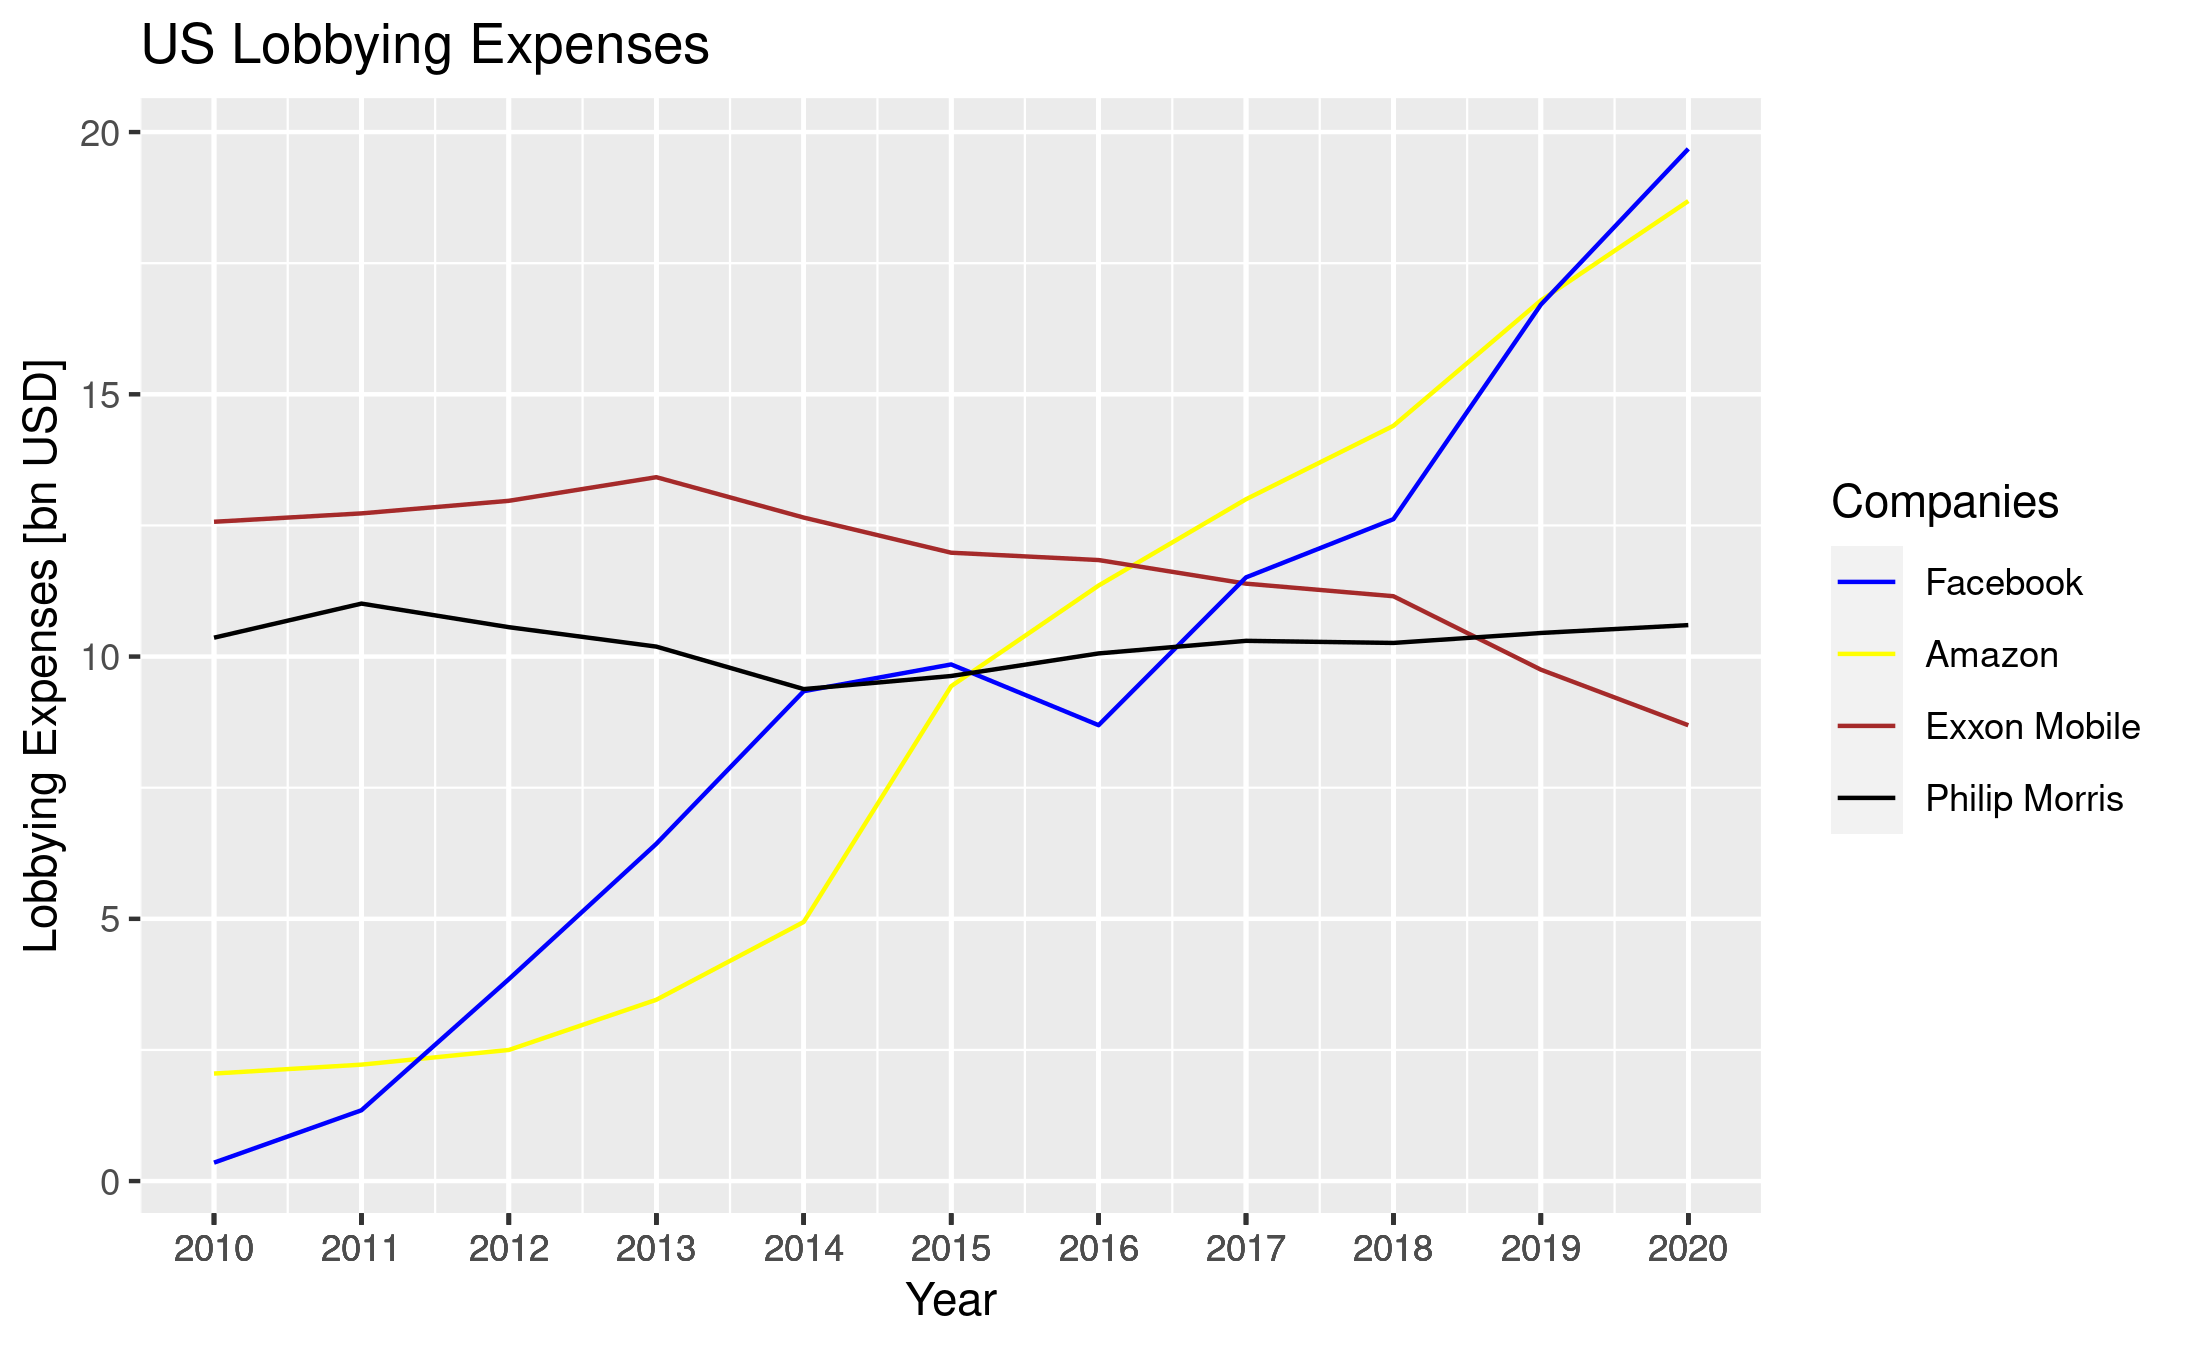
\includegraphics[width=\textwidth]{figures/Lobbying_Expenditures.png}
    \caption{Lobbying Expenditures of: Facebook, Amazon, Exxon Mobile, and Philip Morris over Time, reproduced from \citep{chung_big_2021} with data from \textit{The Center for Responsive Politics} (\href{https://www.opensecrets.org/}{www.opensecrets.org}).}
    \label{fig:lob_exp}
\end{figure}